% SC2008 --- Chapter 1: Overview (History, Layers, Encapsulation) --- 0->100 ground-up
\chapter{Overview: History, Layers, and Encapsulation}
\label{ch:overview}

\begin{quote}
\emph{``The Internet is not a single network, but a network of networks.''} --- Every photo you send, every video call, rides on a few simple ideas: layered abstractions, addresses, and encapsulation. This chapter builds those ideas from zero intuition to precise definitions.
\end{quote}

\noindent\fbox{\parbox{\dimexpr\linewidth-2\fboxsep-2\fboxrule}{%
\textbf{From zero: no networking background assumed.} We define every term from first principles---hosts, packets, protocols, delays, layers---with pictures before formalism. Intuition comes first, then the definition, then the example. The only prerequisites are SC1004 (vectors/matrices for later queueing intuition) and SC2000 (basic probability for later performance reasoning); nothing from them is assumed without explanation. Later chapters depend only on what is built here.}}

\section*{Learning Outcomes}
After this chapter you will be able to:
\begin{enumerate}[label=(L\arabic*)]
    \item describe the Internet as a network of networks and the role of hosts, routers, links, and protocols;
    \item sketch the history from ARPANET to the modern Internet and explain packet switching versus circuit switching;
    \item compare the OSI 7-layer and Internet 5-layer models and articulate service, interface, and protocol;
    \item explain encapsulation and demultiplexing as a packet traverses the protocol stack;
    \item compute end-to-end delay from transmission, propagation, processing, and queueing components.
\end{enumerate}

% ============================================================
\section{What Is a Network? Intuition First}
\label{sec:what-is-network}
Think of sending a letter by post. You write the message, put it in an envelope with the destination address, drop it at a post office, and the postal network routes it hop by hop. The recipient opens the envelope and reads the message. A computer network does the same, but the ``envelope'' is a \emph{packet}, the ``post offices'' are \emph{routers}, and the ``roads'' are \emph{links} (copper, fibre, radio).

Formally, a network is a graph of \emph{nodes} (hosts and routers) connected by \emph{links}. A \emph{host} (end system) runs applications---your laptop, phone, server. A \emph{router} forwards packets toward their destination. An \emph{Internet} (lowercase) is any network of networks; the \emph{Internet} (capitalized) is the global public one governed by IETF standards. Communication obeys a \emph{protocol}: a precise format plus rules for message exchange---exactly like postal conventions. Without a protocol, bits are just noise.

\begin{definition}[Protocol and packet]
A \emph{protocol} defines the format and order of messages and the actions taken on transmission and receipt. A \emph{packet} is the unit of data that carries a payload plus headers added by protocols.
\end{definition}

\subsection{Addresses and Names}
Every host needs an address, just as every house needs a postal address. On the Internet that address is an \emph{IP address} (e.g., \texttt{155.69.0.1}); humans prefer \emph{names} (e.g., \texttt{www.ntu.edu.sg}) because they are memorable. A directory service (DNS, Ch.~2) translates names to addresses. Within a host, a \emph{port number} picks which application gets the packet---like an apartment number inside a building. Together, IP plus port name a socket endpoint uniquely.
\begin{remark}[Why two levels?]
IP gets the packet to the right \emph{host}; the port gets it to the right \emph{process} on that host. Without ports, a server could run only one application. With 16-bit ports ($0$--$65535$), many services share one machine: Web on 80, mail on 25, DNS on 53.
\end{remark}

Two switching ideas compete for how the network shares links. \emph{Circuit switching} (old telephone) reserves a whole path before talking---like booking an entire railway track. \emph{Packet switching} chops data into packets that each find their way independently and share links statistically---like cars merging on a highway. The Internet chose packet switching because it uses links efficiently when traffic is bursty. Bursty means many idle gaps between bursts; reserving a whole circuit would leave it empty most of the time.

\subsection{Delay, Loss, and Throughput}
A packet suffers four delays on each hop: (i) \emph{processing} (router examines header), (ii) \emph{queueing} (waits behind earlier packets), (iii) \emph{transmission} ($L/R$: $L$ bits at link rate $R$~bps), and (iv) \emph{propagation} ($d/s$: distance $d$ at speed $s\approx 2\times10^{8}$~m/s in fibre). Total nodal delay $d_{\text{nodal}}=d_{\text{proc}}+d_{\text{queue}}+d_{\text{trans}}+d_{\text{prop}}$.

\begin{lstlisting}[language=Python, caption={End-to-end delay: intuition to formula.}]
# Each hop adds four delays. Transmission is L/R, propagation is d/s.
def nodal_delay(L_bits, R_bps, d_m, s_mps=2e8, d_proc=0.001, d_queue=0.002):
    d_trans = L_bits / R_bps          # seconds to push bits onto link
    d_prop  = d_m / s_mps              # seconds to propagate
    return d_proc + d_queue + d_trans + d_prop

# Example: 1500-byte packet, 10 Mbps, 1000 km fibre
print(nodal_delay(1500*8, 10e6, 1e6)) # ~0.0092 s per hop
# Add hops and you get end-to-end delay.
\end{lstlisting}

Throughput is the bottleneck rate along the path: $\min_i R_i$. If your access link is 50~Mbps but the core is 10~Gbps, you get 50~Mbps. queueing makes delay random; loss happens when a router buffer overflows---a taste of SC2000 queueing theory we quantify later.

\subsection{A First Example: Sending a Photo}
Suppose you send a 8~Mbit photo from NTU to a friend in London via three hops. Each link is 20~Mbps and 3000~km. Transmission per hop is $8/20=0.4$~s; propagation per hop is $3\times10^{6}/2\times10^{8}=0.015$~s. Three hops give $\approx 3\times(0.4+0.015)=1.245$~s ignoring queueing---transmission dominates. For a 40-byte ACK, transmission is $320/20\times10^{6}=16~\mu$s and propagation dominates instead. This size-dependent crossover is why small packets feel ``latency-bound'' and large transfers feel ``bandwidth-bound.''

\begin{remark}[Delay versus throughput]
Students often conflate delay with throughput. A high-throughput fibre can still have large propagation delay (e.g., Singapore to London $\approx 70$~ms). You can pour water faster (throughput) but water still takes time to travel the pipe (delay). Interactive voice needs low delay; bulk backup needs high throughput.
\end{remark}

Try \texttt{traceroute} (or \texttt{ping}) to see hops and RTTs live: each line is one router, each time is $2\times d_{\text{prop}}+d_{\text{queue}}$. Variation across pings reveals queueing.

% ============================================================
\subsection{Access, Core, and Edge}
The edge is where hosts live (homes, phones, data centres). Access networks connect edge to core: residential fibre/DSL, WiFi, cellular. The core is the mesh of high-speed routers and fibres that interconnect access networks. Logically, the Internet is edge plus access plus core; physically, most bytes travel a few core hops. Content delivery networks (CDNs) push copies to the edge to cut delay---a preview of caching in Ch.~2.

\section{A Brief History: From ARPANET to the Internet}
\label{sec:history}
Why did the Internet win? It stayed simple at the core and pushed complexity to the edges. That principle was learned incrementally.

\begin{figure}[h]
\centering
\resizebox{\linewidth}{!}{%
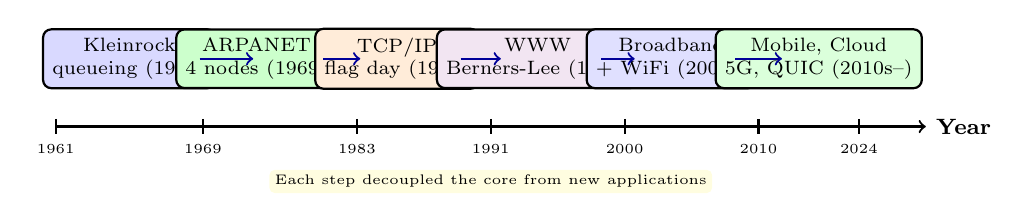
\begin{tikzpicture}[every node/.style={font=\scriptsize}, xscale=0.85, yscale=0.82]
\draw[thick, ->] (0,0) -- (13,0) node[right, font=\footnotesize\bfseries] {Year};
\foreach \x/\yr in {0/1961,2.2/1969,4.5/1983,6.5/1991,8.5/2000,10.5/2010,12/2024} {
  \draw[thick] (\x,0.12)--(\x,-0.12) node[below, font=\tiny] {\yr};
}
\node[draw, thick, fill=blue!15, rounded corners=3pt, minimum width=2.0cm, minimum height=0.65cm, align=center] at (1.1,1.05) {Kleinrock\\queueing (1961)};
\node[draw, thick, fill=green!20, rounded corners=3pt, minimum width=2.0cm, minimum height=0.65cm, align=center] at (3.0,1.05) {ARPANET\\4 nodes (1969)};
\node[draw, thick, fill=orange!15, rounded corners=3pt, minimum width=1.9cm, minimum height=0.65cm, align=center] at (5.1,1.05) {TCP/IP\\flag day (1983)};
\node[draw, thick, fill=violet!10, rounded corners=3pt, minimum width=1.9cm, minimum height=0.65cm, align=center] at (7.2,1.05) {WWW\\Berners-Lee (1991)};
\node[draw, thick, fill=blue!12, rounded corners=3pt, minimum width=1.9cm, minimum height=0.65cm, align=center] at (9.2,1.05) {Broadband\\+ WiFi (2000s)};
\node[draw, thick, fill=green!14, rounded corners=3pt, minimum width=1.9cm, minimum height=0.65cm, align=center] at (11.4,1.05) {Mobile, Cloud\\5G, QUIC (2010s--)};
\draw[->, thick, blue!60!black] (2.15,1.05)--(2.95,1.05);
\draw[->, thick, blue!60!black] (4.0,1.05)--(4.55,1.05);
\draw[->, thick, blue!60!black] (6.05,1.05)--(6.65,1.05);
\draw[->, thick, blue!60!black] (8.15,1.05)--(8.65,1.05);
\draw[->, thick, blue!60!black] (10.15,1.05)--(10.85,1.05);
\node[font=\tiny, align=center, fill=yellow!12, rounded corners=2pt, inner sep=2pt] at (6.5,-0.85) {Each step decoupled the core from new applications};
\end{tikzpicture}}%
\caption{Internet timeline: theory $\to$ first packet-switched network $\to$ universal TCP/IP $\to$ World Wide Web $\to$ ubiquitous broadband and wireless. Each box keeps the core simple; innovation happens at the edges.}
\label{fig:internet-timeline}
\end{figure}

Key moments: 1961 Kleinrock used queueing theory (SC2000) to model packet delays. 1969 ARPANET linked four universities with packet switching. The 1970s produced TCP/IP---one narrow waist that any link technology could carry. 1983 was ``flag day'' when ARPANET switched permanently to TCP/IP. 1991 Tim Berners-Lee added the Web on top, proving the layering idea: no change to routers was needed. The 2000s brought broadband and WiFi; the 2010s brought smartphones, clouds, and encrypted transports like QUIC. The pattern: a simple, universal core plus smarter edges.

\subsection{Packet versus Circuit: A First Trade-off}
Circuit switching guarantees rate but wastes capacity when the user is idle. Packet switching shares statistically: if 10 users each need 10~Mbps only 10\% of the time, a 100~Mbps packet-switched link carries them with small queueing, whereas circuit switching would need $10\times10=100$~Mbps reserved anyway but leave 90\% idle. The price is variable delay and occasional loss.

\begin{example}[Why packet switching won]
A telephone call holds the circuit even during silence. Web browsing is silent 90\% of the time between clicks. Packet switching lets hundreds of browsers share the same link and only contend when they actually send---statistical multiplexing. When contention is rare, queueing stays small and efficiency soars. When everyone clicks at once, queue builds and we need congestion control (Ch.~4).
\end{example}

% ============================================================
\section{Layered Architecture: Service, Interface, Protocol}
\label{sec:layers}
Intuition first: imagine needing a document translated from English to Japanese via French. One translator does English$\leftrightarrow$French, another French$\leftrightarrow$Japanese. Each translator only talks to the adjacent layer and offers a \emph{service} (``I translate French'') via an \emph{interface} (``give me French text''). How the translation is done internally is the \emph{protocol} inside the layer. Networking stacks layers the same way: each layer offers a service to the one above and uses the service below.

\begin{figure}[h]
\centering
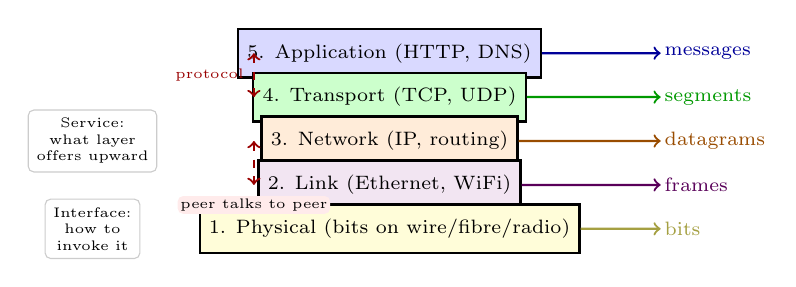
\begin{tikzpicture}[scale=0.82, every node/.style={font=\scriptsize}]
\node[draw, thick, fill=blue!15, minimum width=3.2cm, minimum height=0.62cm] (app) at (0,2.5) {5. Application (HTTP, DNS)};
\node[draw, thick, fill=green!20, minimum width=3.2cm, minimum height=0.62cm] (tr) at (0,1.82) {4. Transport (TCP, UDP)};
\node[draw, thick, fill=orange!15, minimum width=3.2cm, minimum height=0.62cm] (net) at (0,1.14) {3. Network (IP, routing)};
\node[draw, thick, fill=violet!10, minimum width=3.2cm, minimum height=0.62cm] (link) at (0,0.46) {2. Link (Ethernet, WiFi)};
\node[draw, thick, fill=yellow!15, minimum width=3.2cm, minimum height=0.62cm] (phy) at (0,-0.22) {1. Physical (bits on wire/fibre/radio)};
\draw[->, thick, blue!60!black] (app.east) -- (4.2,2.5) node[right, fill=white, inner sep=1pt] {messages};
\draw[->, thick, green!60!black] (tr.east) -- (4.2,1.82) node[right, fill=white, inner sep=1pt] {segments};
\draw[->, thick, orange!60!black] (net.east) -- (4.2,1.14) node[right, fill=white, inner sep=1pt] {datagrams};
\draw[->, thick, violet!70!black] (link.east) -- (4.2,0.46) node[right, fill=white, inner sep=1pt] {frames};
\draw[->, thick, yellow!60!black] (phy.east) -- (4.2,-0.22) node[right, fill=white, inner sep=1pt] {bits};
\node[font=\tiny, align=center, fill=white, rounded corners=2pt, inner sep=3pt, draw=gray!40] at (-4.6,1.14) {Service:\\what layer\\offers upward};
\node[font=\tiny, align=center, fill=white, rounded corners=2pt, inner sep=3pt, draw=gray!40] at (-4.6,-0.22) {Interface:\\how to\\invoke it};
\draw[<->, thick, red!60!black, dashed] (-2.1,2.5) -- (-2.1,1.82) node[midway, left, font=\tiny] {protocol};
\draw[<->, thick, red!60!black, dashed] (-2.1,1.14) -- (-2.1,0.46);
\node[font=\tiny, fill=red!8, rounded corners=2pt, inner sep=1pt] at (-2.1,0.15) {peer talks to peer};
\end{tikzpicture}
\caption{The Internet 5-layer stack. Each layer encapsulates the payload from above, adds its header, and uses the service below. The OSI 7-layer model splits Application into Application/Presentation/Session; TCP/IP merges them.}
\label{fig:layer-stack}
\end{figure}

\begin{definition}[Service, interface, protocol]
A \emph{service} is what a layer offers to the layer above. An \emph{interface} is how that service is invoked (e.g., socket API between Application and Transport). A \emph{protocol} is the distributed algorithm peers at the same layer use to implement the service.
\end{definition}

The Internet collapses OSI's seven layers into five: Application, Transport, Network, Link, Physical. Presentation and Session functions (encryption, compression) live inside the Application when needed. This minimal waist is why the same IP runs over fibre, WiFi, or satellite, and why HTTP, DNS, and streaming apps all share the same network---each app only interacts with Transport via sockets.

Why layering? Three benefits: (i) \emph{modularity}---replace WiFi with Ethernet without touching TCP; (ii) \emph{abstraction}---each layer hides complexity below; (iii) \emph{reuse}---one Transport serves many applications. Cost: headers add overhead and layering can hide useful information (e.g., wireless losses look like congestion to TCP).

\begin{remark}[The hourglass]
The Internet is an hourglass: many applications on top, many link technologies below, and a single narrow waist---IP---in the middle. Any app that speaks IP runs over any link that carries IP. That waist is why innovation at the edges (new apps) and at the bottom (new radios) can evolve independently.
\end{remark}

% ============================================================
\subsection{Throughput Revisited: Bottlenecks}
Think of a water pipe with three segments of diameters 10~cm, 2~cm, 10~cm: throughput is limited by the narrowest segment (2~cm), no matter how wide the others are. On the Internet the bottleneck is usually the access link (your home WiFi or phone), not the core. When many flows share a link, each gets a fair share---congestion control (Ch.~4) negotiates that share dynamically.

\section{Encapsulation and Demultiplexing}
\label{sec:encapsulation}
When Host~A sends ``Hello'' to Host~B, the message descends the stack; each layer wraps it with a header (and sometimes a trailer) and passes the larger unit down. On receipt, each layer unwraps its header and demultiplexes upward.

\begin{figure}[h]
\centering
\resizebox{\linewidth}{!}{%
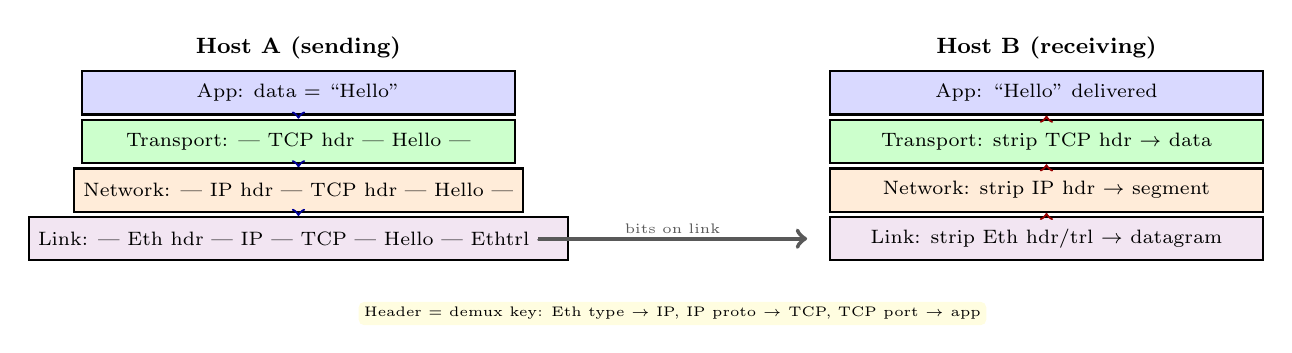
\begin{tikzpicture}[every node/.style={font=\scriptsize}, scale=0.95]
% Sending side
\node[font=\footnotesize\bfseries] at (0,3.2) {Host A (sending)};
\node[draw, thick, fill=blue!15, minimum width=5.5cm, minimum height=0.55cm] (a5) at (0,2.6) {App: data = ``Hello''};
\node[draw, thick, fill=green!20, minimum width=5.5cm, minimum height=0.55cm] (a4) at (0,1.95) {Transport: | TCP hdr | Hello |};
\node[draw, thick, fill=orange!15, minimum width=5.5cm, minimum height=0.55cm] (a3) at (0,1.30) {Network: | IP hdr | TCP hdr | Hello |};
\node[draw, thick, fill=violet!10, minimum width=5.5cm, minimum height=0.55cm] (a2) at (0,0.65) {Link: | Eth hdr | IP | TCP | Hello | Ethtrl |};
\draw[->, thick, blue!60!black] (a5)--(a4); \draw[->, thick, blue!60!black] (a4)--(a3); \draw[->, thick, blue!60!black] (a3)--(a2);
% Channel
\draw[->, ultra thick, gray!70!black] (3.2,0.65) -- (6.8,0.65) node[midway, above, font=\tiny, fill=white, inner sep=1pt] {bits on link};
% Receiving side
\node[font=\footnotesize\bfseries] at (10,3.2) {Host B (receiving)};
\node[draw, thick, fill=violet!10, minimum width=5.5cm, minimum height=0.55cm] (b2) at (10,0.65) {Link: strip Eth hdr/trl $\to$ datagram};
\node[draw, thick, fill=orange!15, minimum width=5.5cm, minimum height=0.55cm] (b3) at (10,1.30) {Network: strip IP hdr $\to$ segment};
\node[draw, thick, fill=green!20, minimum width=5.5cm, minimum height=0.55cm] (b4) at (10,1.95) {Transport: strip TCP hdr $\to$ data};
\node[draw, thick, fill=blue!15, minimum width=5.5cm, minimum height=0.55cm] (b5) at (10,2.6) {App: ``Hello'' delivered};
\draw[->, thick, red!60!black] (b2)--(b3); \draw[->, thick, red!60!black] (b3)--(b4); \draw[->, thick, red!60!black] (b4)--(b5);
% Demux annotation
\node[font=\tiny, align=center, fill=yellow!12, rounded corners=2pt, inner sep=2pt] at (5, -0.35) {Header = demux key: Eth type $\to$ IP, IP proto $\to$ TCP, TCP port $\to$ app};
\end{tikzpicture}}%
\caption{Encapsulation on sending and decapsulation on receiving. Each header names which upper-layer protocol should receive the payload (demultiplexing).}
\label{fig:encapsulation}
\end{figure}

\emph{Demultiplexing} uses header fields as keys: Ethernet's EtherType says ``this is IP'', IP's Protocol says ``this is TCP'', TCP's destination port says ``deliver to the Web server, not the mail server.'' Without these keys, the receiver could not know which application should get the bytes.

\begin{definition}[PDU and overhead]
Each layer names its packet: Application \emph{message}, Transport \emph{segment} (TCP) or \emph{datagram} (UDP), Network \emph{datagram}, Link \emph{frame}. The header-to-payload ratio is overhead; for a 20-byte TCP header carrying 1460~bytes of data, overhead is $20/1480\approx1.35\%$---layering is cheap.
\end{definition}

\begin{lstlisting}[language=Python, caption={Layering as encapsulation: each layer wraps the payload.}]
class Layer:
    def __init__(self, name, header): self.name=name; self.header=header
    def encapsulate(self, payload): return f"|{self.header}|{payload}|"
    def decapsulate(self, packet): return packet.split("|")[2]  # strip one header

stack = [Layer("App",""), Layer("Transport","TCP"), Layer("Network","IP"), Layer("Link","ETH")]
payload = "Hello"
for layer in reversed(stack):  # top-down encapsulation
    if layer.header: payload = layer.encapsulate(payload)
print(payload)  # |ETH||IP||TCP|Hello|||
# Receiving reverses the order, each layer checking its header.
\end{lstlisting}

% ============================================================
\begin{example}[Ping as a layering lab]
Run \texttt{ping -c 3 www.google.com}: each ICMP echo is encapsulated as IP datagram, then Ethernet frame on WiFi. The reported time is $2(d_{\text{prop}}+d_{\text{queue}})+d_{\text{proc}}$ round-trip. Try \texttt{ping -s 1000} versus \texttt{ping -s 100} to see transmission delay grow with packet size, and \texttt{traceroute} to see per-hop delays.
\end{example}

\section{Chapter Notes}
Layering follows the end-to-end principle (Saltzer--Reed--Clark, 1984). History from Leiner et al.\ \emph{Brief History of the Internet} and Kurose--Ross. Delay taxonomy is standard: queueing analysis uses SC2000 probability in Ch.~3. Wireshark lets you see encapsulation live---capture a ping and peel headers.

% ============================================================
\section{Exercises}
\label{sec:ch01-exercises}
\begin{enumerate}[label=E1.\arabic*, leftmargin=*, itemsep=0.8em]
    \item \textbf{Circuit vs.\ packet.} Ten users each need 1~Mbps when active (active 20\% of time, independent). A 4~Mbps circuit link reserves per active user. How many users can a circuit link support? What blocking probability would a packet link face with all ten sharing 4~Mbps? Why does bursty traffic favour packet switching?
    \item \textbf{Delay arithmetic.} A 12\,000-bit packet crosses two links: $R_1=2$~Mbps, $R_2=5$~Mbps, each 500~km ($s=2\times10^{8}$~m/s), $d_{\text{proc}}=1$~ms, queueing negligible. Compute $d_{\text{trans}}$ per link, $d_{\text{prop}}$ per link, and total end-to-end delay. Which term dominates?
    \item \textbf{Layering trade-offs.} Your teammate proposes merging Transport and Network into one layer ``to save headers.'' Give two modularity or reuse arguments against this and one scenario where cross-layer information would help. What invariant does layering protect?
    \item \textbf{Demultiplexing keys.} A host runs a Web server (TCP port 80), a DNS resolver (UDP port 53), and video streaming (UDP port 5004). When an IP datagram arrives with Protocol=6 (TCP) and dst port 80, trace the demultiplexing chain from Link to Application and state which header field is used at each step.
    \item \textbf{Wireshark peek.} Capture or sketch a ping (ICMP over IP over Ethernet). List the three headers you see, their sizes, and which field tells Ethernet that the payload is IP and which tells IP that the payload is ICMP.
\end{enumerate}
% End of Chapter 1